%File: formatting-instructions-latex-2023.tex
%release 2023.0
\documentclass[letterpaper]{article} % DO NOT CHANGE THIS
\usepackage{aaai23}  % DO NOT CHANGE THIS
\usepackage{times}  % DO NOT CHANGE THIS
\usepackage{helvet}  % DO NOT CHANGE THIS
\usepackage{courier}  % DO NOT CHANGE THIS
\usepackage[hyphens]{url}  % DO NOT CHANGE THIS
\usepackage{graphicx} % DO NOT CHANGE THIS
\urlstyle{rm} % DO NOT CHANGE THIS
\def\UrlFont{\rm}  % DO NOT CHANGE THIS
\usepackage{natbib}  % DO NOT CHANGE THIS AND DO NOT ADD ANY OPTIONS TO IT
\usepackage{caption} % DO NOT CHANGE THIS AND DO NOT ADD ANY OPTIONS TO IT
\frenchspacing  % DO NOT CHANGE THIS
\setlength{\pdfpagewidth}{8.5in}  % DO NOT CHANGE THIS
\setlength{\pdfpageheight}{11in}  % DO NOT CHANGE THIS
%
% These are recommended to typeset algorithms but not required. See the subsubsection on algorithms. Remove them if you don't have algorithms in your paper.
\usepackage{algorithm}
\usepackage{algorithmic}

%
% These are are recommended to typeset listings but not required. See the subsubsection on listing. Remove this block if you don't have listings in your paper.
\usepackage{newfloat}
\usepackage{listings}
\DeclareCaptionStyle{ruled}{labelfont=normalfont,labelsep=colon,strut=off} % DO NOT CHANGE THIS
\lstset{%
	basicstyle={\footnotesize\ttfamily},% footnotesize acceptable for monospace
	numbers=left,numberstyle=\footnotesize,xleftmargin=2em,% show line numbers, remove this entire line if you don't want the numbers.
	aboveskip=0pt,belowskip=0pt,%
	showstringspaces=false,tabsize=2,breaklines=true}
\floatstyle{ruled}
\newfloat{listing}{tb}{lst}{}
\floatname{listing}{Listing}
%
% Keep the \pdfinfo as shown here. There's no need
% for you to add the /Title and /Author tags.
\pdfinfo{
/TemplateVersion (2023.1)
}

% DISALLOWED PACKAGES
% \usepackage{authblk} -- This package is specifically forbidden
% \usepackage{balance} -- This package is specifically forbidden
% \usepackage{color (if used in text)
% \usepackage{CJK} -- This package is specifically forbidden
% \usepackage{float} -- This package is specifically forbidden
% \usepackage{flushend} -- This package is specifically forbidden
% \usepackage{fontenc} -- This package is specifically forbidden
% \usepackage{fullpage} -- This package is specifically forbidden
% \usepackage{geometry} -- This package is specifically forbidden
% \usepackage{grffile} -- This package is specifically forbidden
% \usepackage{hyperref} -- This package is specifically forbidden
% \usepackage{navigator} -- This package is specifically forbidden
% (or any other package that embeds links such as navigator or hyperref)
% \indentfirst} -- This package is specifically forbidden
% \layout} -- This package is specifically forbidden
% \multicol} -- This package is specifically forbidden
% \nameref} -- This package is specifically forbidden
% \usepackage{savetrees} -- This package is specifically forbidden
% \usepackage{setspace} -- This package is specifically forbidden
% \usepackage{stfloats} -- This package is specifically forbidden
% \usepackage{tabu} -- This package is specifically forbidden
% \usepackage{titlesec} -- This package is specifically forbidden
% \usepackage{tocbibind} -- This package is specifically forbidden
% \usepackage{ulem} -- This package is specifically forbidden
% \usepackage{wrapfig} -- This package is specifically forbidden
% DISALLOWED COMMANDS
% \nocopyright -- Your paper will not be published if you use this command
% \addtolength -- This command may not be used
% \balance -- This command may not be used
% \baselinestretch -- Your paper will not be published if you use this command
% \clearpage -- No page breaks of any kind may be used for the final version of your paper
% \columnsep -- This command may not be used
% \newpage -- No page breaks of any kind may be used for the final version of your paper
% \pagebreak -- No page breaks of any kind may be used for the final version of your paperr
% \pagestyle -- This command may not be used
% \tiny -- This is not an acceptable font size.
% \vspace{- -- No negative value may be used in proximity of a caption, figure, table, section, subsection, subsubsection, or reference
% \vskip{- -- No negative value may be used to alter spacing above or below a caption, figure, table, section, subsection, subsubsection, or reference

\setcounter{secnumdepth}{0} %May be changed to 1 or 2 if section numbers are desired.

% The file aaai23.sty is the style file for AAAI Press
% proceedings, working notes, and technical reports.
%

% Title

% Your title must be in mixed case, not sentence case.
% That means all verbs (including short verbs like be, is, using,and go),
% nouns, adverbs, adjectives should be capitalized, including both words in hyphenated terms, while
% articles, conjunctions, and prepositions are lower case unless they
% directly follow a colon or long dash
\title{Comparison of Deep Neural Network and Support Vector Machine on Image Classification Tasks }
\author{
    %Authors
    % All authors must be in the same font size and format.
    Qin He
}
\affiliations{
    %Afiliations
    % If you have multiple authors and multiple affiliations
    % use superscripts in text and roman font to identify them.
    % For example,

    % Sunil Issar, \textsuperscript{\rm 2}
    % J. Scott Penberthy, \textsuperscript{\rm 3}
    % George Ferguson,\textsuperscript{\rm 4}
    % Hans Guesgen, \textsuperscript{\rm 5}.
    % Note that the comma should be placed BEFORE the superscript for optimum readability

    Department of Statistical Science, Duke University \\
    % email address must be in roman text type, not monospace or sans serif
    qin.he696@duke.edu
%
% See more examples next
}






\begin{document}
\maketitle

\begin{abstract}
This study aims to present an analysis on the performances of the support vector machine and deep neural networks on image classifications, and how are the performances impacted by the size of sample data available. The task in this study is primarily on training models that can effectively  recognize hand-written digits from the MNIST database.The MNIST dataset consists of handwritten digits images which are diverse and highly distorted. Two separate models  are trained on the same the entire dataset first, and then trained on a subset of 3000 samples . The first model is a multi-layer deep neural networks with convolution layers. The second model is a support vector machine model developed with radial basis function kernel. The result demonstrates that both model are able to achieve high accuracy on when trained on the full dataset with CNN model slightly better than SVM. However, the performance of SVM is better than that of CNN when trained on the small dataset.
\end{abstract}

\section{Introduction}
Computer Vision(CV) is among one of the most popular topics in the research of machine learning and artificial intelligence. The ultimate goal is to enable machines to  understand and automate tasks that the human visual system can do. Specifically, it aims to find ways to make machines extract meaningful information from visual data, such as images or stream of video. In the past, when computational power is limited, few problem can be practical solved by fitting neural networks, as its training process is generally computationally heavy. Instead, many of the traditional algorithms does not require extensive computing power. Support Vector Machine(SVM) is one of the popular choice among them. Nowadays, most of the state-art-of works on computer vision tasks are based on deep learning models. DL is used to solve varieties of difficult problems including image colourization, classification, segmentation and detection. DL methods such as Convolutional Neural Networks (CNNs) mostly improve prediction performance using big data and plentiful computing resources and have pushed the boundaries of what was possible. However, it is not easy to conclude that the noval DL models dominated the traditional SVM models under any circumstances. Especially, there are debates on if training multi-layer convolutional neural network is a over kill when many of the traditional models can yield comparable results but at lower cost. This study aims to compare the performances of both algorithms on a well-studied dataset. The model will be fitted on the full dataset and on a sampled subset. It is expected that large neural is able to output model with high accuracy with sufficient amount of data. However, when the size of dataset is limited, it is unclear if large NN model can still outperform the traditional SVM model.

\section{Data}
The dataset used in this study is MNIST dataset.It is a large database of handwritten digits that is commonly used for training various image processing systems. It was created by "re-mixing" the samples from NIST's original datasets. It contains 60,000 training images and 10,000 testing images. One of the important characteristics of MNIST dataset is that it is a clean dataset without any unexpected missing values, and hence there is no concern on bias introduced by systematic missingness. In addition,One of the main concerns in many of the machine learning and deep learning tasks is unbalanced data, but the labels in MNIST data is balanced well, as illustrated by figure 1. \\\\
In addition to data quality, the other reason to use this dataset is that it has been well studied, and there are a number of models proven to perform well on this dataset. This is to exclude potential bias in performances comparison brought poorly designed models. There are a lot of tricks for training moth SVM and CNN models. Especially for deep learning models, there is a large range of potential hyperparameters to tune, and there are almost infinite number of combinations to stack layers of neurons and apply tricks like dropout or poolings. In addition, the tuning process of CNN models generally takes considerable amount of time. Hence, if this study is conducted on datasets that are not thoroughly studied, it is possible that the differences in performances are not caused by the model but rather on insufficient tuning or poor design of the model. Instead, this study includes two sets of parameter and an architecture of CNN models that has been shown to be able to achieve over 98 percent accuracy. \\


\begin{figure}[h]
\caption{Distribution of Labels}
\centering
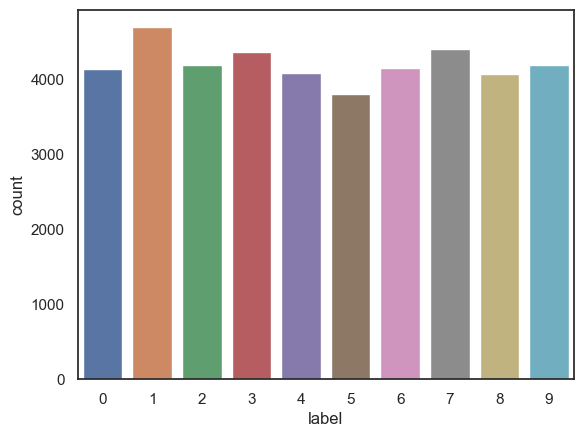
\includegraphics[width=8cm]{labelCount}  
\end{figure}

\section{Convolutional neural network}
A Convolutional Neural Network, also known as CNN or ConvNet, is a class of neural networks that specializes in processing data that has a grid-like topology, such as an image. A digital image is a binary representation of visual data. It contains a series of pixels arranged in a grid-like fashion that contains pixel values to denote how bright and what color each pixel should be.

CNNs models are attempts to mimic the architecture of human brains, and how the visual inputs are processed by human brians. Just as each neuron responds to stimuli only in the restricted region of the visual field called the receptive field in the biological vision system, each neuron in a CNN processes data only in its receptive field as well. The layers are arranged in such a way so that they detect simpler patterns first (lines, curves, etc.) and more complex patterns (faces, objects, etc.) further along.
A CNN typically has three layers: a convolutional layer, a pooling layer, and a fully connected layer, as illustrated by Figure 2.

\begin{figure}[h]
\caption{CNN Model}
\centering
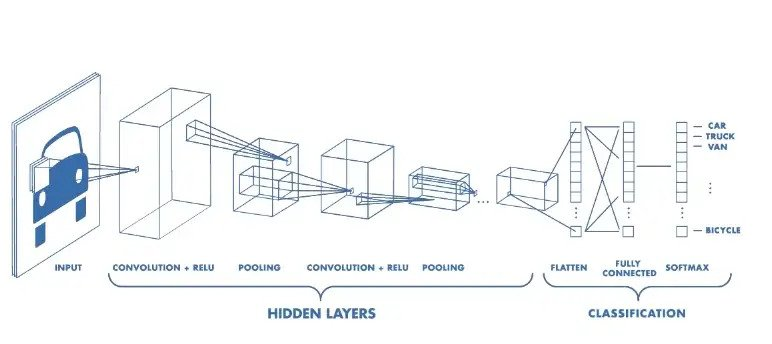
\includegraphics[width=8cm]{cnns.jpg}  
\end{figure}

\\
The convolution layer is the core building block of the CNN. It carries the main portion of the network’s computational load.
This layer performs a dot product between two matrices, where one matrix is the set of learnable parameters otherwise known as a kernel, and the other matrix is the restricted portion of the receptive field. The kernel is spatially smaller than an image but is more in-depth. This means that, if the image is composed of three (RGB) channels, the kernel height and width will be spatially small, but the depth extends up to all three channels.During the forward pass, the kernel slides across the height and width of the image-producing the image representation of that receptive region. This produces a two-dimensional representation of the image known as an activation map that gives the response of the kernel at each spatial position of the image. The sliding size of the kernel is called a stride.

Trivial neural network layers use matrix multiplication by a matrix of parameters describing the interaction between the input and output unit. This means that every output unit interacts with every input unit. However, convolution neural networks have sparse interaction. This is achieved by making kernel smaller than the input e.g., an image can have millions or thousands of pixels, but while processing it using kernel we can detect meaningful information that is of tens or hundreds of pixels. This means that we need to store fewer parameters that not only reduces the memory requirement of the model but also improves the statistical efficiency of the model. In addition, in a traditional neural network, each element of the weight matrix is used once and then never revisited, while convolution network has shared parameters i.e., for getting output, weights applied to one input are the same as the weight applied elsewhere. Due to parameter sharing, the layers of convolution neural network will have a property of equivalence to translation. It says that if we changed the input in a way, the output will also get changed in the same way.


\section{Implementation}
There are many well-established packages for building deep learning models. This study uses Tensorflow to define, build and train a multi-layer CNN model. The model includes a convolution layer, a dropout layer to avoid over fitting as well as a max pooling layer. Besides layers specification, dropouts and pooling, activation function is also an important factor when designing the model. For this model, the output layer uses a softmax function as the task is on classifying multiple labels. A mathematical expression of Softmax Function is defined below.
\begin{eqnarray}
\sigma(y_{i}) = \left(\frac{e^{y_{i}}}{ \sum\limits_{j} e^{y_{j}}}\right)
j = 1,...,n
\end{eqnarray}
Besides the output layers, other layers uses RELU function as the activation function. The RELU function is a simple calculation that returns the value provided as input directly, or the value 0.0 if the input is 0 or less. \\

In addition, a data augmentation technique is used to generate additional data for training purpose. This is a commonly used trick to improve the performance of deep learning models. In this study, additional data points are generated by applying a series of transformation on the images, and expect that they are equivalent to the originals. For example, an rotated 8 should still be classified as 8, and in fact it bears the label as the original one. 
\begin{figure}[h]
\caption{ Rotated Imagel}
\centering
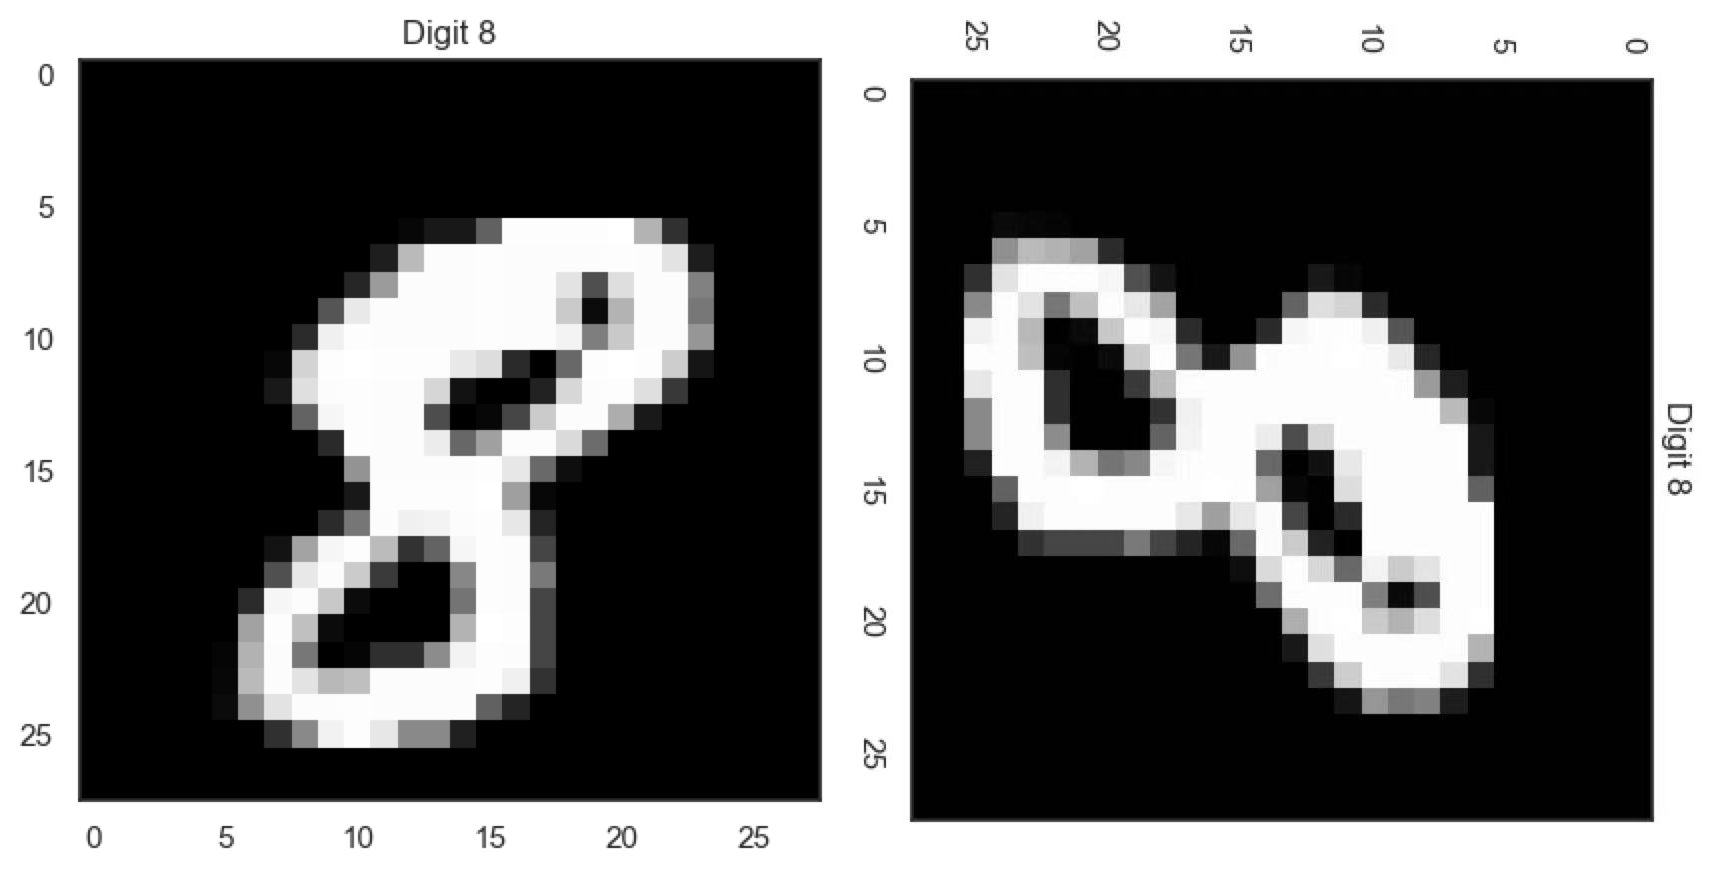
\includegraphics[width=8cm]{eight.jpg}  
\end{figure}


\section{Support Vector Machine}
An popular alternative choice for deep learning models on computer vision task is support vector machine. Support vector machine is an algorithm used widely in classification problems in machine learning. SVM creates a hyperplane, plane that separates the features and classifies the new input data point based on its value. The SVM algorithm finds its optimal decision boundary by maximizing the margin. When the data is non-linearly separable. Mathematically, this can be expressed as \\
\begin{align*}
\max_{w,b} \frac{2}{||w||} \\s.t.\ y_{i}(w^{T}x_{i} + b) \geq 1, i=1,2,...,m; \\ L(w,b,\alpha)=\frac{1}{2}||w||^2 + \sum^{m}_{i=1}a_{i}(1-y_{i}(w^{T}x_{i} + b))       
\end{align*}
 
SVM can use kernels to convert low dimensional non-linearly separable data points into high dimensional linearly separable data points. Widely known kernels include polynomial, radial basis function, and sigmoid kernels. In this study, all the model is trained using RBF kernel. The model is implemented using Sci-Kit Learn(Sklearn)'s SVC function in Python


\begin{figure}[h]
\caption{CNN Mode Performance}
\centering
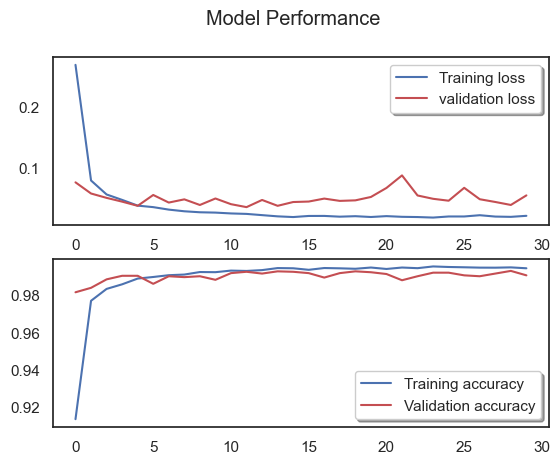
\includegraphics[width=8cm]{performance.jpg}  
\end{figure}

\begin{figure}[h]
\caption{CNN Mode With Data Augmentation Performance}
\centering
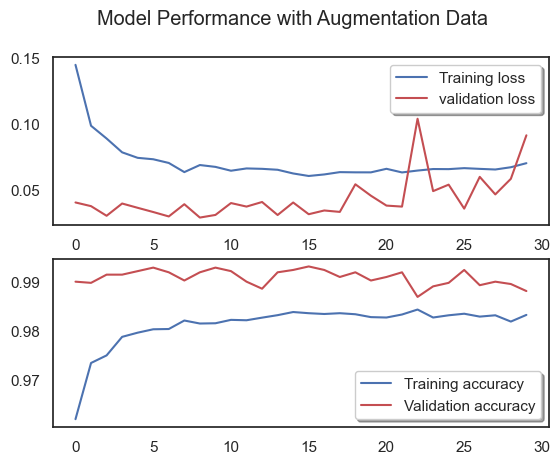
\includegraphics[width=8cm]{performanceAug.jpg}  
\end{figure}

\begin{figure}[h]
\caption{CNN Mode Performance}
\centering
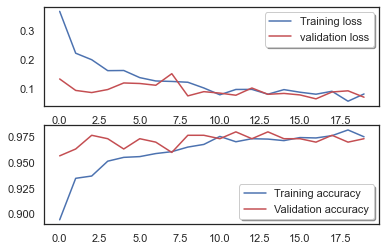
\includegraphics[width=8cm]{small_simple.jpg}  
\end{figure}

\begin{figure}[h]
\caption{CNN Mode With Data Augmentation Performance}
\centering
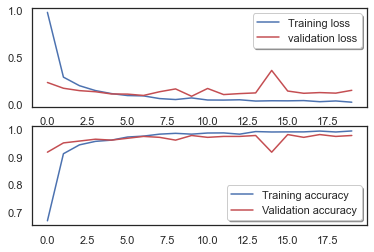
\includegraphics[width=8cm]{small_aug.jpg}  
\end{figure}
\section{Result}
The study is divided into 2 steps. Both steps share identical model structures, hyper-parameters, and train-test split ratio. The MNIST data has a built-in split for train and test data. However, this study will focus on the splitting on training data, and the the performance of both algorithms on the validation data will be evaluated. At step 1, after both SVM and CNN model are developed, the entire MNIST data is fed into the model to train the model. Both loss and accuracy are recorded at each epoch.
As Figure 4 shows, both accuracy and loss of the CNN model converges quickly over the epochs, and the model is able to achieve over 98 percent validation accuracy after 30 epochs. In addition, there is a clear sign of decreasing in validation loss and increasing in accuracy over the epochs. Even if there is sudden spike in the middle, the loss eventually falls by the end of training session, and hence there is no sign of overfitting. 
Figure 5 shows similar results but on the model with data augmentation. The accuracy achieved is higher than the model without it. The pattern is very similar to the previous one with the exception that the sudden increase of loss in the middle is much higher. It may indicates that the model is overfitting, but it converts to little impact on the validation accuracy. Both graph illustrates that CNN model is able to achieve high accuracy given sufficient amount of data. Meanwhile, the SVM model is only able to achieve around 96 percent accuracy on the validation dataset. It showcase that the CNN model can outperform the SVM model on the entire dataset. On the second step, both models are retrained on a subset of the MNIST database with 3000 samples. The results of CNN models are illustrated in Figure 6 and 7. It shows a significant drop in accuracy in both approach. Even if data augmentation can produce new data sample, the samples are drawn from a more limited source, and hence the performance is worse. For this part, the SVM also suffers from a drastic drop in performance. It only achieves 91 percent accuracy, and the changes is even larger than that for CNNs. \\
To sum up, CNN, regardless of with data augmentations or not, can outperform SVM under both full and small data scenario. However, it is also notable that SVM's achievable accuracy is not significantly lower than that of CNNs. SVM is able to perform considerably well in both cases, and it is much more computationally efficient to train when compared with CNNs. Maybe sometimes it is unnecessary to spend such large cost for training when SVM can do reasonably well with lower cost.
\\
\newpage

\section{}
\mbox{}
\nocite{*}
\bibliographystyle{amsplain}
\bibliography{aaai23_new}

\subsection{Code}
All the code , data and files for this study is available at  \href{https://github.com/QinHE325/BioStats823FinalProject}.
\end{document}

